\documentclass[../../docenti.tex]{subfiles}

\begin{document}
\section{Introduzione}

\subsection{Obiettivi}
L'obiettivo di questa unità didattica è quello di consolidare le conoscenze acquisite nel corso di programmazione a blocchi applicandole ad un nuovo ambito, quello della programmazione di microcontrollori.\\
Le logiche di programmazione sono quelle viste in classe, il microcontrollore aggiunge la possibilità di interagire con il mondo esterno attraverso sensori e attuatori, consentendo esercizi e progetti più interattivi e vicini alla vita di tutti i giorni. 


\subsection{Materiali}
Gli esercizi proposti nei capitoli seguenti sono stati pensati per essere svolti da studenti divisi in gruppi di 2-3 persone.

Ogni gruppo necessita di un computer con connessione ad internet. Sarebbe ottimale avere a disposizione un microbit per ogni gruppo, ma è possibile lavorare con il dispositivo simulato presente nell'editor online e mettere a disposizione alcuni dispositivi per test da passare tra gli studenti.

\subsection{Prerequisiti}
Per poter svolgere gli esercizi proposti è necessario che gli studenti abbiano già una conoscenza di base di programmazione a blocchi e di programmazione in generale.\\
Prima di ogni esercizio verranno elencati i concetti chiave che si assume lo studente conosca e quelli che si vuole introdurre (o rafforzare).

\newpage
\subsection{Micro:Bit}
 MicroBit è un microcontrollore sviluppato da BBC, un'azienda britannica, per insegnare le basi della programmazione e dell'informatica.

\begin{figure}[H]
 	\centering
 	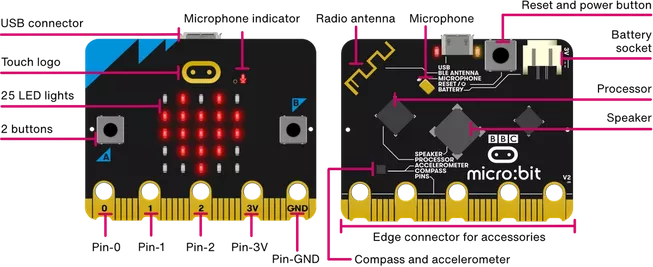
\includegraphics[width=0.8\linewidth]{microbitScheme.png}
 	\caption{Sensori ed attuatori MicroBit versione 1 \parencite{MicrobitOverview}}
 	\label{fig:microbit}
\end{figure}

Il dispositivo è dotato di un display (una griglia di 5x5 LED), due pulsanti e molti sensori\footnote{Una lista completa di sensori e attuatori con esempi di utilizzo è disponibile al seguente indirizzo: \url{https://microbit.org/get-started/user-guide/overview}} tra cui:
\begin{itemize}
	\item accelerometro
	\item giroscopio
	\item sensore di luminosità
	\item sensore di rumore
\end{itemize}

\subsection{Make:Code}
MakeCode è un editor online per la programmazione di microcontrollori.\\



\newpage
\begin{itemize}
	\item Introduzione a microbit 
	\item Introduzione a MakeCode
\end{itemize}
\end{document}